\documentclass[12pt]{article}
\usepackage{latexsym,amssymb,amsmath} % for \Box, \mathbb, split, etc.
% \usepackage[]{showkeys} % shows label names
\usepackage{cite} % sorts citation numbers appropriately
\usepackage{path}
\usepackage{url}
\usepackage{verbatim}
\usepackage[pdftex]{graphicx}

% horizontal margins: 1.0 + 6.5 + 1.0 = 8.5
\setlength{\oddsidemargin}{0.0in}
\setlength{\textwidth}{6.5in}
% vertical margins: 1.0 + 9.0 + 1.0 = 11.0
\setlength{\topmargin}{0.0in}
\setlength{\headheight}{12pt}
\setlength{\headsep}{13pt}
\setlength{\textheight}{625pt}
\setlength{\footskip}{24pt}

\renewcommand{\textfraction}{0.10}
\renewcommand{\topfraction}{0.85}
\renewcommand{\bottomfraction}{0.85}
\renewcommand{\floatpagefraction}{0.90}

\usepackage{accents}
\newcommand{\ubar}[1]{\underaccent{\bar}{#1}}
\makeatletter
\setlength{\arraycolsep}{2\p@} % make spaces around "=" in eqnarray smaller
\makeatother
\usepackage{stackengine}
% change equation, table, figure numbers to be counted inside a section:
\numberwithin{equation}{section}
\numberwithin{table}{section}
\numberwithin{figure}{section}

% begin of personal macros
\newcommand{\half}{{\textstyle \frac{1}{2}}}
\newcommand{\eps}{\varepsilon}
\newcommand{\myth}{\vartheta}
\newcommand{\myphi}{\varphi}

\newcommand{\IN}{\mathbb{N}}
\newcommand{\IZ}{\mathbb{Z}}
\newcommand{\IQ}{\mathbb{Q}}
\newcommand{\IR}{\mathbb{R}}
\newcommand{\IC}{\mathbb{C}}
\newcommand{\Real}[1]{\mathrm{Re}\left({#1}\right)}
\newcommand{\Imag}[1]{\mathrm{Im}\left({#1}\right)}
\DeclareRobustCommand{\brkbinom}{\genfrac[]{0pt}{}}
\newcommand{\norm}[2]{\|{#1}\|_{{}_{#2}}}
\newcommand{\abs}[1]{\left|{#1}\right|}
\newcommand{\ip}[2]{\left\langle {#1}, {#2} \right\rangle}
\newcommand{\der}[2]{\frac{\partial {#1}}{\partial {#2}}}
\newcommand{\dder}[2]{\frac{\partial^2 {#1}}{\partial {#2}^2}}
\usepackage{enumitem}
\newcommand{\nn}{\mathbf{n}}
\newcommand{\xx}{\mathbf{x}}
\newcommand{\uu}{\mathbf{u}}
\usepackage{tikz}
\usetikzlibrary{arrows}
\usetikzlibrary{positioning}
\usepackage{titlesec}
\newcommand{\junk}[1]{{}}
\usepackage{sectsty}
\usepackage{xcolor}
\newcommand*{\bfrac}[2]{\genfrac{}{}{0pt}{}{#1}{#2}}
\newcommand\myatop[2]{\left[{{#1}\atop#2}\right]} % "wrapper macro"
\usepackage{array}
\usepackage{multirow}
\usepackage{amsmath}
\DeclareMathOperator*{\argmax}{arg\,max}
\DeclareMathOperator*{\argmin}{arg\,min}
\makeatletter
\renewcommand*\env@matrix[1][\arraystretch]{%
	\edef\arraystretch{#1}%
	\hskip -\arraycolsep
	\let\@ifnextchar\new@ifnextchar
	\array{*\c@MaxMatrixCols c}}
\makeatother

\makeatletter
\renewcommand*\env@matrix[1][*\c@MaxMatrixCols c]{%
	\hskip -\arraycolsep
	\let\@ifnextchar\new@ifnextchar
	\array{#1}}
\makeatother

\definecolor{darkblue}{rgb}{0,0,0.4}
\usepackage[colorlinks = true,
linkcolor = darkblue,
urlcolor  = darkblue,
citecolor = darkblue,
anchorcolor = darkblue]{hyperref}
% set two lengths for the includegraphics commands used to import the plots:
\newlength{\fwtwo} \setlength{\fwtwo}{0.45\textwidth}
% end of personal macros

\begin{document}
\DeclareGraphicsExtensions{.jpg}

\begin{center}
\textsc{\Large Statistical Pattern Recognition} \\[2pt]
	\textsc{\large Assignment 4}\\
	\vspace{0.5cm}
  Ali Gholami \\[6pt]
  Department of Computer Engineering \& Information Technology\\
  Amirkabir University of Technology  \\[6pt]
  \def\UrlFont{\em}
  \url{https://aligholamee.github.io}\\
    \href{mailto:aligholami7596@gmail.com}{\textit{aligholami7596@gmail.com}}
\end{center}

\begin{abstract}

\end{abstract}

\subparagraph{Keywords.} \textit{KNN Classifier, Kernel Density Estimation.}

\section{Kernel Density Estimation \& KNN Estimation}
Given dataset $ X = 2, 3, 4, 4, 4, 5, 5, 10, 11, 11, 11, 12, 14, 16 $ use Parzen windows to estimate density $p(x)$ at $x = 5$ and $x = 12$; assuming $h = 4$ in the following conditions.
\begin{enumerate}[label=(\alph*)]
	\item If you use standard kernel function
	\[ K(u) =
	\begin{cases}
	1      & \quad |u| \leq \frac{1}{2}\\
	0  & \quad o.w.
	\end{cases}
	\]


	\item If you use Gaussian Kernel, $N(0, 10)$.
	
	\item For the same dataset and the same sample points, i.e. $x = 5$ and $x = 12$, estimate the density using KNN approach. Take $ K = 5$ in your estimations.

\end{enumerate}

\subsection*{Solution}
\begin{enumerate}[label=(\alph*)]
	\item We'll use (1.1) to estimate the density using different kernels.
	\begin{equation}
	\hat{p}_{(x)} = \frac{1}{n*h^d} \sum_{i = 1}^{k}\Phi(\frac{x - x_i}{h})
	\end{equation}
	In this case, we'll compute the distance of each of the given points from our dataset. For every distance less than 2 we'll consider the effect of that point in our estimation.
	$$
		x = 5\ \ \ \rightarrow\ \ \ \hat{p}_{(x)} = \frac{1}{14 * 4} * (6) = \frac{3}{28} = 0.107
	$$
	Doing the same for the point $x = 12$ and we'll have the following results:
	$$
		x = 12\ \ \ \rightarrow\ \ \ \hat{p}_{(x)} = \frac{1}{14 * 4} * (6) = \frac{3}{28} = 0.107
	$$
	
	\item In this case, the value of items in the $\sum$ are no longer 1. They will have different outputs, specially on the center of the curve. This can lead to an smoother and more realistic estimation of the density. The Gaussian Kernel equation is given in (1.2).
	\begin{equation}
		\phi(u) = \frac{1}{\sqrt{2\pi}}\exp(\frac{-u^2}{2})
	\end{equation}
	
	$$
		x = 5\ \ \ \rightarrow\ \ \ \hat{p}_{(x)} = \frac{1}{14 * 4} * \frac{1}{\sqrt{2\pi}} (\exp(-2) + 3\exp(\frac{-1}{2}) + 2)) = 0.028
	$$
	
	$$
		x = 12\ \ \ \rightarrow\ \ \ \hat{p}_{(x)} = \frac{1}{14 * 4} * \frac{1}{\sqrt{2\pi}} (2\exp(-2) + 3\exp(\frac{-1}{2}) + 1)) = 0.021
	$$
	
	\item In this case, we have to consider the window size as a dynamic variable. In case $h = 2$ then $x = 4$, $x = 4$, $x = 4$ and $x = 5$ will be in our window of estimation as well as the centered point $x = 5$ (K = 5). To estimate the density we'll have the following equation:
	$$
		x = 5\ \ \ \rightarrow\ \ \ \hat{p}_{(x)} = \frac{1}{14 * 2} * (5) = 0.178
	$$
	Note that we have considered the kernel to be the same as part a. In the second case, choosing the $h = 2$ yields 5 points.
	$$
	x = 12\ \ \ \rightarrow\ \ \ \hat{p}_{(x)} = \frac{1}{14 * 2} * (5) = 0.178
	$$
\end{enumerate}

\section{Parzen Windows \& KNN Estimation}
Consider the following training set drawn from an unknown density $f(x)$:
$$
	X = \{ 0.01, 0.12, 0.19, 0.32, 0.41, 0.48\}
$$
\begin{enumerate}[label=(\alph*)]
		
	\item	Let $\phi(x) = N(1, 0)$. Find and sketch the Parzen Windows estimate for the values of $h_n$ of $0.1$ and $1.0$.
	\begin{equation}
	\hat{f_n}_{(x)} = \frac{1}{n*h_n} \sum_{i = 1}^{k}\Phi(\frac{x - x_i}{h_n})
	\end{equation}
	
	
	\item Find and sketch the 3-nearest neighbor estimate of $f(x)$.
\end{enumerate}

\section*{Solution}

\begin{enumerate}[label=(\alph*)]
	\item For each point in our dataset, we'll center the Gaussian Kernel and add the values of these kernels. Here are the computations in case that $h_n = 0.1$.
	$$
	\hat{f_n}_{(x = 0.01)} = \frac{1}{6*0.1} *1  = 1.66 \ \ \ \ \hat{f_n}_{(x = 0.12)} = \frac{1}{6*0.1} * 1= 1.66
	$$

	$$
	\hat{f_n}_{(x = 0.19)} = \frac{1}{6*0.1} * 1 = 1.66 \ \ \ \ \hat{f_n}_{(x = 0.32)} = \frac{1}{6*0.1} * 1 = 1.66
	$$
	$$
	\hat{f_n}_{(x = 0.41)} = \frac{1}{6*0.1} * 1 = 1.66\ \ \ \ 	\hat{f_n}_{(x = 0.48)} = \frac{1}{6*0.1} * 1 = 1.66
	$$
	As denoted above, estimation will give 0 for all of the points in the dataset with $h_n = 0.1$. We can understand that, the window size has been chosen too small that no point is being considered by the estimator. Note that the $h = 0.1$ will be divided by 2 (Being symmetric) and the neighborhood of each given point in the dataset is checked with a diameter of $0.05$. In this case, non of the windows contained other points. Since we have considered the point itself having an effect on the density (As in previous problem), we'll consider them here also.
	
	In the second case, the window size is $h_n = 1.0$. For each point in the dataset, if we put a window of size 1.0 on that point, all other points are included in the window. We can understand that in this case, the window size is too large. $f(x)$ estimation is given below.
	
	$$
		\hat{f_n}_{(x =0.01)} = \frac{1}{6*0.1} * (exp(0) + exp(\frac{-0.0121}{2}) +
		 exp(\frac{-0.0324}{2}) + exp(\frac{-0.0961}{2}) + 
	$$
	$$
	exp(\frac{-0.16}{2}) + exp(\frac{-0.2209}{2}) = 0.95
	$$	
	This procedure is same for all of the given points in the dataset. In the case of window size of 0.1, the estimation results is given in the figure 2.1.
	\begin{figure}[!h]\centering
		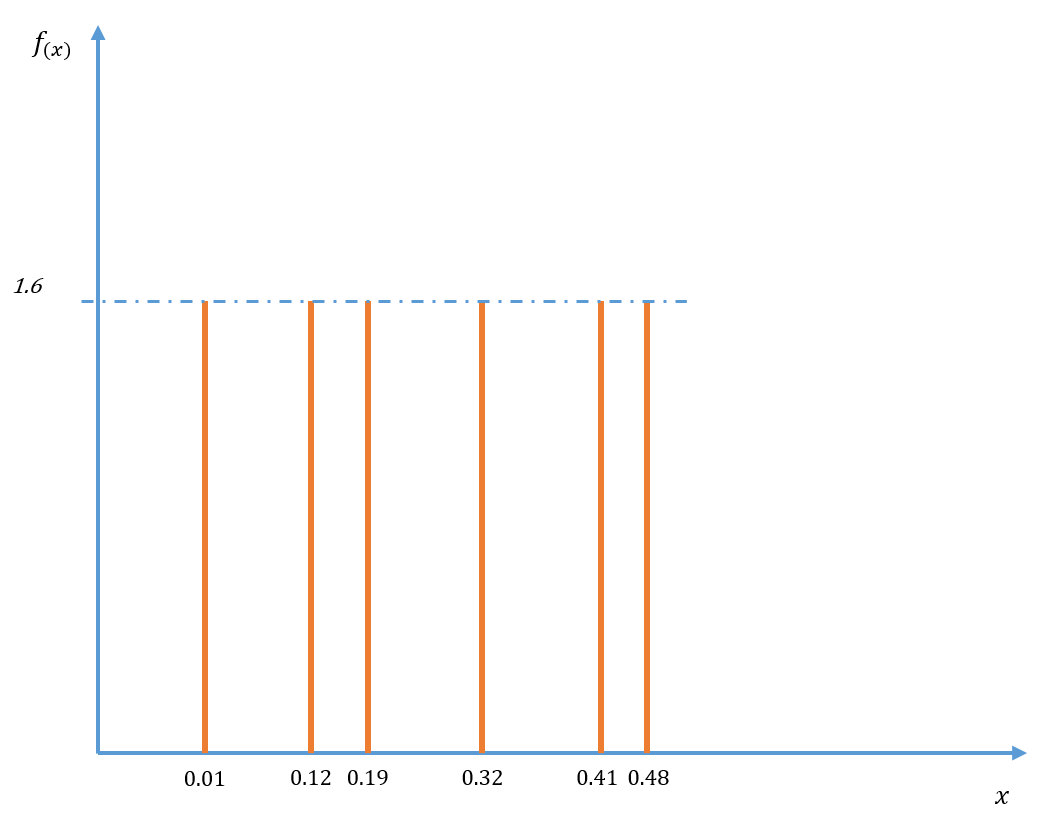
\includegraphics[width=0.6\textwidth]{2_a_1.PNG}
		\caption{Kernel Estimation of f(x) with $h_n = 0.1$.}
		\label{pl1}
	\end{figure}
\end{enumerate}



\end{document} 

